\documentclass[a4paper,UTF8]{article}
\usepackage{ctex}
\usepackage[margin=1.25in]{geometry}
\usepackage{color}
\usepackage{graphicx}
\usepackage{amssymb}
\usepackage{amsmath}
\usepackage{amsthm}
\usepackage{enumerate}
\usepackage{bm}
\usepackage{hyperref}
\usepackage{pgfplots}
\usepackage{epsfig}
\usepackage{color}
\usepackage{tcolorbox}
\usepackage{mdframed}
\usepackage{lipsum}


\usepackage{natbib}
\newmdtheoremenv{thm-box}{myThm}
\newmdtheoremenv{prop-box}{Proposition}
\newmdtheoremenv{def-box}{定义}

\setlength{\evensidemargin}{.25in}
\setlength{\textwidth}{6in}
\setlength{\topmargin}{-0.5in}
\setlength{\topmargin}{-0.5in}
% \setlength{\textheight}{9.5in}
%%%%%%%%%%%%%%%%%%此处用于设置页眉页脚%%%%%%%%%%%%%%%%%%
\usepackage{fancyhdr}                                
\usepackage{lastpage}                                           
\usepackage{layout}                                             
\footskip = 10pt 
\pagestyle{fancy}                    % 设置页眉                 
\lhead{2022年春季}                    
\chead{机器学习理论研究导引}                                                
% \rhead{第\thepage/\pageref{LastPage}页} 
\rhead{大作业}                                                                                               
\cfoot{\thepage}                                                
\renewcommand{\headrulewidth}{1pt}  			%页眉线宽,设为0可以去页眉线
\setlength{\skip\footins}{0.5cm}    			%脚注与正文的距离           
\renewcommand{\footrulewidth}{0pt}  			%页脚线宽,设为0可以去页脚线

\makeatletter 									%设置双线页眉                                        
\def\headrule{{\if@fancyplain\let\headrulewidth\plainheadrulewidth\fi%
		\hrule\@height 1.0pt \@width\headwidth\vskip1pt	%上面线为1pt粗  
		\hrule\@height 0.5pt\@width\headwidth  			%下面0.5pt粗            
		\vskip-2\headrulewidth\vskip-1pt}      			%两条线的距离1pt        
	\vspace{6mm}}     								%双线与下面正文之间的垂直间距              
\makeatother  

%%%%%%%%%%%%%%%%%%%%%%%%%%%%%%%%%%%%%%%%%%%%%%
\numberwithin{equation}{section}
%\usepackage[thmmarks, amsmath, thref]{ntheorem}
\newtheorem{myThm}{myThm}
\newtheorem*{myDef}{Definition}
\newtheorem*{mySol}{Solution}
\newtheorem*{myProof}{Proof}
\newtheorem*{myRemark}{备注}
\renewcommand{\tilde}{\widetilde}
\renewcommand{\hat}{\widehat}
\newcommand{\indep}{\rotatebox[origin=c]{90}{$\models$}}
\newcommand*\diff{\mathop{}\!\mathrm{d}}

\usepackage{multirow}

%--

%--
\begin{document}
	\title{机器学习理论研究导引\\
		大作业}
	\author{陈晟\, MG21330006\, 计算机科学与技术} 
	\date{}
	\maketitle
	%%%%%%%% 注意: 使用XeLatex 编译可能会报错,请使用 pdfLaTex 编译 %%%%%%%
	
	\section*{作业提交注意事项}
	\begin{tcolorbox}
		\begin{enumerate}
			\item[(1)] 本次作业提交截止时间为~\textcolor{red}{\textbf{2022/07/10  23:59:59}}, 截止时间后不再接收作业, 本次作业记零分; 
			\item[(2)] 作业提交方式:使用此~LaTex~模板书写解答,只需提交编译生成的~pdf~文件,将~pdf~文件上传到以下ftp服务器的指定位置:
			\newline 地址:sftp://210.28.132.67:22,用户名:mlt2022,密码:mltspring2022@nju
			\newline 文件夹位置:/C:/Users/mlt2022/hw\_submissions/hw6\_submission/  ;
			\item[(3)] pdf 文件命名方式:学号-姓名-作业号-v版本号, 例~ MG1900000-张三-6-v1;如果需要更改已提交的解答,请在截止时间之前提交新版本的解答,并将版本号加一;
			\item[(4)] 未按照要求提交作业,或~pdf~命名方式不正确,将会被扣除部分作业分数. 
		\end{enumerate}
	\end{tcolorbox}
	
	\begin{abstract}
		
		此处为文章摘要
		
	\end{abstract}
	
	
	\newpage
	\section{图神经网络(GNN)简介}
	在计算机科学中,图是由节点和边两部分组成的一种数据结构。图G可以通过节点集合V和它包含的边E来进行描述。如下图所示:
	
	\begin{figure}[ht]
		\centering
		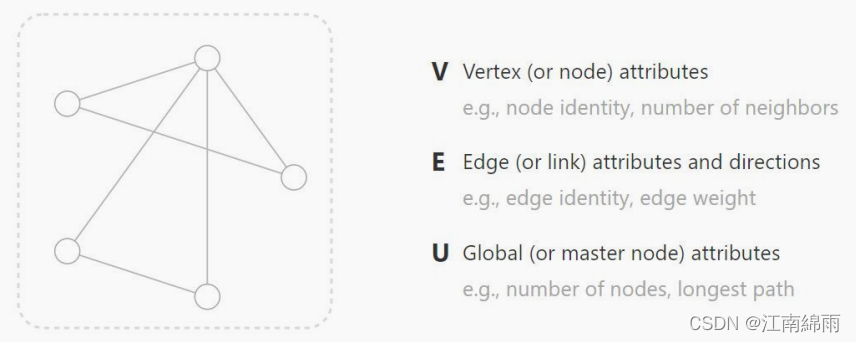
\includegraphics[scale=0.4]{1.png}
		\caption{图结构的表示}
		\label{fig:label}
	\end{figure}
	
	图(graph)是一种数据结构,图神经网络(Graph Neural Network)应该是深度学习在图结构数据上的一些模型、方法和应用。常见的图结构由节点(node)和边(edge)构成,节点包含了实体(entity)信息,边包含实体间的关系(relation)信息。现在许多学习任务都需要处理图结构的数据,比如引文网络、社交网络、交通网络,物理系统建模(physics system)、学习分子指纹(molecular fingerprints)、蛋白质接口预测(protein interface)以及疾病分类(classify diseases),这些都需要模型能够从图结构的输入中学习相关的知识。
	
	GNN起源于两种动机,一种动机来自于卷积神经网络(CNN),另一种动机来自于图嵌入(graph embedding)。第一种来源于CNN,CNN能够提取出多尺度的局部空间特征,并将它们进行组合来构建更加高级的表示(expressive representations)。如果深入研究CNN和图结构的特点,可以发现CNN的核心特点在于:局部连接(local connection),权重共享(shared weights)和多层叠加(multi-layer)。这些同样在图问题中非常试用,因为图结构是最典型的局部连接结构,其次,共享权重可以减少计算量,另外,多层结构是处理分级模式(hierarchical patterns)的关键。然而,CNN只能在欧几里得数据(Euclidean data),比如二维图片和一维文本数据上进行处理,而这些数据只是图结构的特例而已,对于一般的图结构,可以发现很难将CNN中的卷积核(convolutional filters)和池化操作(pooling operators)迁移到图的操作上。如图2,左图为图像,是比较明显的Euclidean数据,而右图为普通的graph结构。
	
	\begin{figure}[ht]
		\centering
		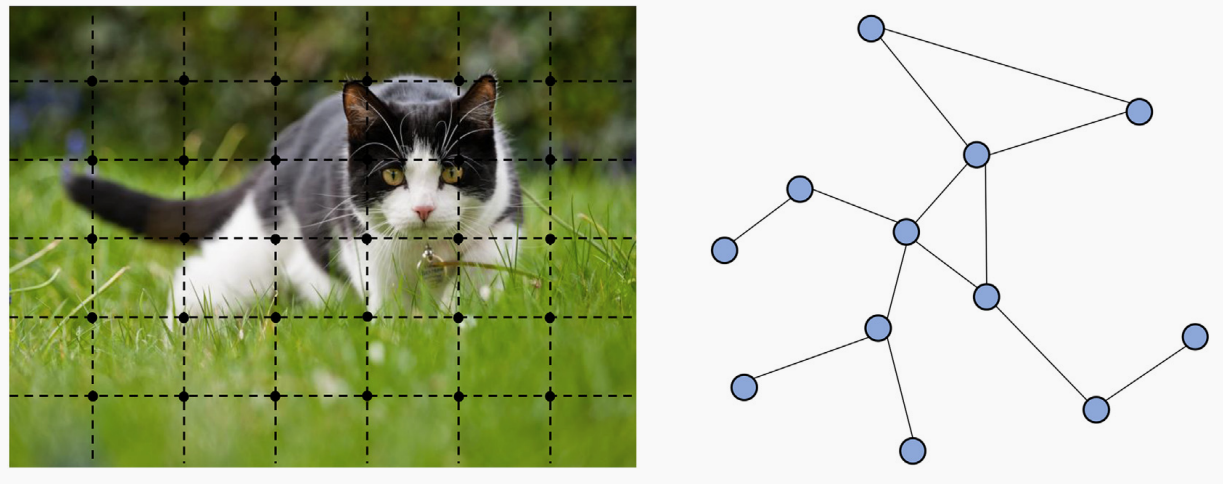
\includegraphics[scale=0.4]{2.png}
		\caption{欧式空间与非欧式空间}
		\label{fig:label}
	\end{figure}
	
	GNN和普通的神经网络相比,具有下列的优势,首先标准的神经网络比如CNN和RNN不能够适当地处理图结构输入,因为它们都需要节点的特征按照一定的顺序进行排列,但是,对于图结构而言,并没有天然的顺序而言,如果使用顺序来完整地表达图的话,那么就需要将图分解成所有可能的序列,然后对序列进行建模,显然,这种方式非常的冗余以及计算量非常大,与此相反,GNN采用在每个节点上分别传播(propagate)的方式进行学习,由此忽略了节点的顺序,相当于GNN的输出会随着输入的不同而不同。
	
	另外,图结构的边表示节点之间的依存关系,然而,传统的神经网络中,依存关系是通过节点特征表达出来的,也就是说,传统的神经网络不是显式地表达中这种依存关系,而是通过不同节点特征来间接地表达节点之间的关系。通常来说,GNN通过邻居节点的加权求和来更新节点的隐藏状态。
	
	最后,就是对于高级的人工智能来说,推理是一个非常重要的研究主题,人类大脑的推理过程基本上都是基于图的方式,这个图是从日常的生活经历中学习得到的。GNN尝试从非结构化数据比如情景图片和故事文本中产生结构化的图,并通过这些图来生成更高级的AI系统。
	
	
	\section{图神经网络的理论发展}
	
	\subsection{图神经网络原理概念}
	
	图神经网络的概念最初由\citep{journal/FScarselli2009} 提出,该论文将现存的神经网络模型扩展到处理图领域的数据。在一个图结构中,每一个节点由它自身的特征以及与其相连的节点特征来定义该节点。GNN的目标是学习得到一个状态的嵌入向量(embedding) $h_v \in \mathcal{R}^s$ ,这个向量包含每个节点的邻居节点的信息,其中, $h_v$ 表示节点 $v$ 的状态向量,这个向量可以用于产生输出 $o_v$ ,比如输出可以是节点的标签,假设 $f$ 是带有参数的函数,叫做局部转化函数(local transition function),这个函数在所有节点中共享,并根据邻居节点的输入来更新节点状态,假设 $g$ 为局部输出函数(local output function),这个函数用于描述输出的产生方式。那么 $h_v$ 和 $o_v$ 按照如下式子产生:
	
	$$
	\begin{gathered}
		\mathbf{h}_{v}=f\left(\mathbf{x}_{v}, \mathbf{x}_{c o[v]}, \mathbf{h}_{n e[v]}, \mathbf{x}_{n e[v]}\right) \\
		\mathbf{o}_{v}=g\left(\mathbf{h}_{v}, \mathbf{x}_{v}\right)
	\end{gathered}
	$$
	其中, $\mathbf{x}_{v} , \mathbf{x}_{c o[v]}, \mathbf{h}_{n e[v] }, \mathbf{x}_{n e[v]} $分别表示节点 $ v$  的特征向量,节点 $ v $ 边的特征向量,节点 $v$ 邻居节点的状态向量和节点 $v$ 邻居节点特征向量。
		假设将所有的状态向量,所有的输出向量,所有的特征向量呈加起来分别使用矩阵 $\mathbf{H}$ , $\mathbf{O}$ , $\mathbf{X}$ 和 $\mathbf{X}_{N}$ 来表示,那么可以得到更加紧凑的表示:
		$$
		\begin{gathered}
			\mathbf{H}=F(\mathbf{H}, \mathbf{X}) \\
			\mathbf{O}=G\left(\mathbf{H}, \mathbf{X}_{N}\right)
		\end{gathered}
		$$
		其中, $F$ 表示全同转化函数(global transition function), $G$ 表示全局输出函数(global output function),分别是所有节点 $f$ 和 $g$ 的咺加形式, $\mathbf{H}$ 是上面第一个方程的不动点,并 且在 $F$ 为收缩映射的假设下 $\mathbf{H}$ 被唯一地定义。根据Banach的不动点定理,GNN使用如下的传 统迭代方法来计算状态参量:
		$$
		\mathbf{H}^{t+1}=F\left(\mathbf{H}^{t}, \mathbf{X}\right)
		$$
		其中, $\mathbf{H}^{t}$ 表示 $\mathbf{H}$ 的第 $t$ 个迭代周期的张量,按照上述方程迭代的系统按照指数级速度收敛 收敛到最终的不动点解。
		在定义好GNN的框架之后,下一个问题就是学习函数 $f$ 和 $g$ 的参数,使用目标信息(使用 $\mathbf{t}_{v}$ 表 示特定节点的标签)来进行监督学习,loss可以定义如下:
		$$
		\text { loss }=\sum_{i=1}^{p}\left(\mathbf{t}_{i}-\mathbf{o}_{i}\right)
		$$
		
		其中,$p$表示监督的节点数量,学习算法使用梯度下降法,整个过程按照如下步骤进行:
		
		状态 $h_v^t$ 按照迭代方程更新$T$ 个轮次,这时得到的$H$ 会接近不动点的解$H(T) \approx H$ ;
		权重$W$的梯度从loss计算得到;
		权重$W$根据上一步中计算的梯度更新。
		
		\subsection{图神经网络强大性的理论分析}
		GNN目前主流的做法是递归迭代聚合一阶邻域表征来更新节点表征,如GCN和GraphSAGE,但这些方法大多是经验主义,缺乏理论去理解GNN到底做了什么,还有什么改进空间。\citep{conf/Keyulu2019}基于Weisfeiler-Lehman(WL) test 视角理论分析了GNN,包括分析了GNN做了什么?在什么条件下GNN可以和WL test一样强大?提出了满足上述一个简单的GNN框架GIN,并在实验中取得预期效果。现在主流GNN变种在捕获图结构上的不足及特性。
		
		Weisfeiler-Lehman(WL) test 是判断两个graph是否具有相同的结构(同构)非常有效的方法,迭代进行以下操作得到节点新标签以判断同构性:
		(初始化:将节点自身id作为标签)
		
		1. 聚合方案:聚合每个节点邻域和自身标签。
		2. 更新节点标签:使用Hash映射节点聚合标签,作为节点新标签。
		同构:如果图G1和G2的顶点和边的数目相同,并且边的连通性相同,则这两个图可以说是同构的,如下图所示。也可以认为G2的顶点是从G1的顶点映射而来的。这是一个具有挑战性的问题:目前还没有已知的多项式时间算法。图同构的Weisfeiler-Lehman(WL)检验是一种有效且计算效率高的检验,它能区分一大类图。
		
		GNN迭代过程和WL test非常相似,受这个启发,\citep{conf/Keyulu2019}提出定理2,证明了 WL test是GNN能力的上限:如果任意G1, G2 是非同构图,如果存在GNN可以将其映射到两个不同的embedding,那么WL test 也能判断G1、G2非同构。
		
		\begin{figure}[ht]
			\centering
			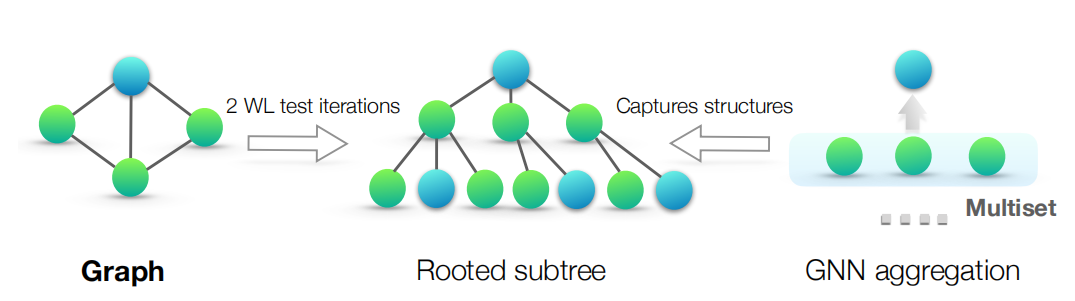
\includegraphics[scale=0.5]{3.png}
			\caption{WL test过程和GNN迭代过程}
			\label{fig:label}
		\end{figure}
		
		对GNN做如下描述,GNN的目标是以图结构数据和节点特征作为输入,以学习到节点(或图)的embedding,用于分类任务。
		
		基于邻域聚合的GNN可以拆分为以下三个模块:
		
		1.Aggregate:聚合一阶邻域特征。
		
		2.Combine:将邻居聚合的特征 与 当前节点特征合并, 以更新当前节点特征。
		
		3. Readout(可选):如果是对graph分类,需要将graph中所有节点特征转变成graph特征。
		
		GNNs 基本思想: 邻域聚集函数+更新函数
		$$
		a_{v}^{(k)}=\operatorname{AGGREGATE}^{(k)}\left(\left\{h_{u}^{(k-1)}: u \in \mathcal{N}(v)\right\}\right), \quad h_{v}^{(k)}=\operatorname{COMBINE}^{(k)}\left(h_{v}^{(k-1)}, a_{v}^{(k)}\right)
		$$
		GraphSAGE 模型:
		$$
		a_{v}^{(k)}=\operatorname{MAX}\left(\left\{\operatorname{ReLU}\left(W \cdot h_{u}^{(k-1)}\right), \forall u \in \mathcal{N}(v)\right\}\right)
		$$
		$$
		W \cdot\left[h_{v}^{(k-1)}, Q^{(k)}\right]
		$$
		GCN模型:
		$$
		h_{v}^{(k)}=\operatorname{ReLU}\left(W \cdot \operatorname{MEAN}\left\{h_{u}^{(k-1)}, \forall u \in \mathcal{N}(v) \cup\{v\}\right\}\right)
		$$
		对于节点分类任务来说,最后迭代的节点表示hv (K) 直接用于预测。对于图分类来说,还需要 READOUT函数将节点向量转化为图像,可以是简单的置换不变函数如求和,或更复杂的图形级池 函数。
		
		为了研究GNN的表示能力,我们分析了什么时候GNN会将两个节点映射到嵌入空间中的同一位置。直观地说,一个最强大的GNN,只有当两个节点具有相同的子树结构,而且子树结构在相应的节点上具有相同的特征时,才会映射两个节点到相同的位置。由于子树结构是通过节点邻域递归定义的(图1),我们可以将分析简化为一个GNN是否将两个邻域(即两个多集)映射到同一个嵌入或表示的问题。一个最强大的GNN将从不映射两个不同的邻域,即多个特征向量集,到相同的表示。这意味着它的聚合方案必须是单射的。因此,我们将GNN的聚合方案抽象为其神经网络能够表示的多集上的一类函数,并分析它们对于多集是否是单射。如果GNN中Aggregate、Combine 和 Readout 函数是单射,GNN可以和WL test 一样强大
		
		$$
		h_{v}^{(k)}=\phi\left(h_{v}^{(k-1)}, f\left(\left\{h_{u}^{(k-1)}: u \in \mathcal{N}(v)\right\}\right)\right)
		$$
		
		其中作用于多集的函数 $f$ 、和都是单射函数。
		2、作用在节点表示 $\{h v(k)\}$ 上的readout函数也是单射函数。
		上述结论只对于可数集有效,节点特征连续的不可数集需要进一步考虑。
		GRAPH ISOMORPHISM NETWORK (GIN)
		$$
		h_{v}^{(k)}=\operatorname{MLP}^{(k)}\left(\left(1+\epsilon^{(k)}\right) \cdot h_{v}^{(k-1)}+\sum_{u \in \mathcal{N}(v)} h_{u}^{(k-1)}\right)
		$$
		$$
		h_{G}=\operatorname{CONCAT}\left(\operatorname{READOUT}\left(\left\{h_{v}^{(k)} \mid v \in G\right\}\right) \mid k=0,1, \ldots, K\right) .
		$$
		
		对上面的公式做两个操作:用单层感知器代替MLPs;用平均或最大池代替和。就可以发现,这些GNN变体被令人惊讶的简单图形所混淆,并且不如WL测试强大。尽管如此,具有平均聚合器(如GCN)的模型在节点分类任务中表现良好。为了更好地理解这一点,我们精确地描述了不同GNN变体可以捕获和不能捕获的图形,并讨论了使用图形学习的含义。1层感知器的行为很像线性映射,因此GNN层退化为简单的邻域特征求和。我们的证明建立在偏差项缺少线性映射的事实上。利用偏差项和足够大的输出维数,单层感知器可能可以区分不同的多集。因此,即使具有1层感知器的GNNs可以在一定程度上将不同的图嵌入到不同的位置,这样的嵌入也可能无法充分捕获结构相似性,并且对于简单的分类器(例如线性分类器)来说很难拟合。
		
		\begin{figure}[ht]
			\centering
			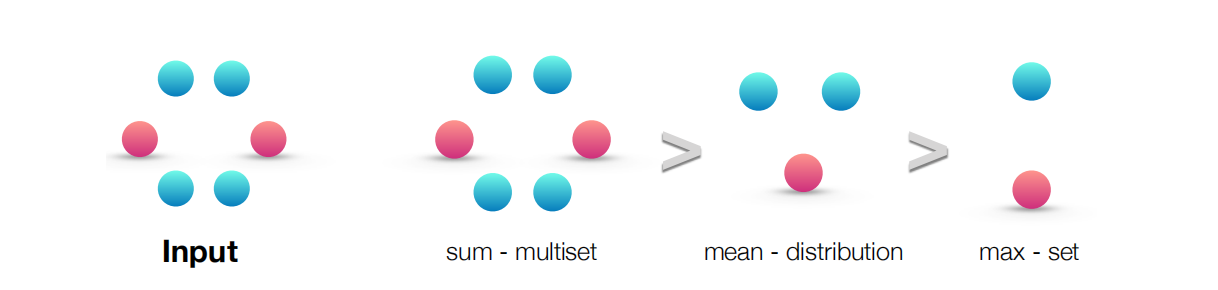
\includegraphics[scale=0.5]{4.png}
			\caption{按表示能力对三个聚合器进行了排序,多集上求和、平均和最大聚合器的表示能力排序。左面板显示输入多集,即要聚合的网络邻居。接下来的三个面板说明了给定聚合器能够捕获的多集的各个方面:sum捕获完整的多集,mean捕获给定类型元素的比例/分布,max聚合器忽略多重性(将多集减少为简单集)}
			\label{fig:label}
		\end{figure}
		
		\begin{figure}[ht]
			\centering
			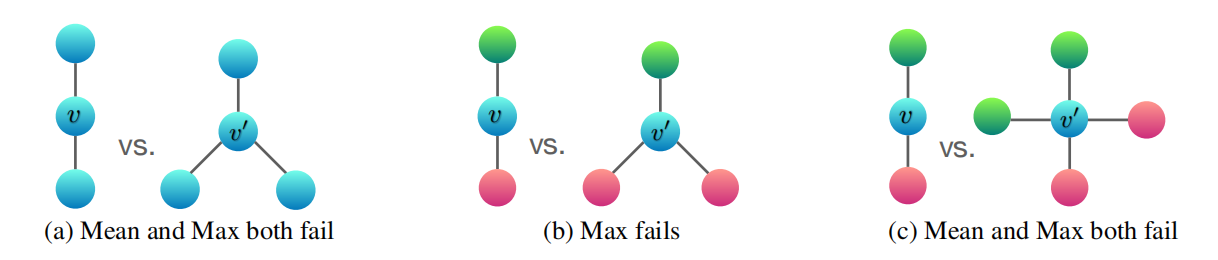
\includegraphics[scale=0.5]{5.png}
			\caption{显示了平均池聚合器和最大池聚合器无法区分的结构对,在这里,节点颜色表示不同的节点特征,我们假设GNNs在与标记为v和v′的中心节点组合之前先聚集邻居}
			\label{fig:label}
		\end{figure}
		
		图4说明了sum可以学习精确的结构信息,mean偏向学习分布信息,max偏向学习有代表性的元素信息。
		
		图5就说明了mean和max 无法区分哪些结构。
		
		图5(a)
		
		mean: 左: $\frac{1}{2}(b+b)=b$ ,右: $\frac{1}{3}(b+b+b)=b \mathrm{~ , 无 法 区 分 。 ~}$
		
		$\max$ : 左:b,右:b 无法区分
		
		sum:左:2b,右: $3 b$ ,可以区分。
		
		图5(b)
		
		mean: 左: $\frac{1}{2}(r+g)$ ,右: $\frac{1}{3}(g+2 r)$ ,可以区分。
		
		$\max :$ 左: $\max (r, g)$ ,右: $\max (g, r, r)$ ,无法区分。
		
		sum: 左: $r+g$ ,右: $2 r+g$ ,可以区分。
		
		图5(c)
		
		mean: 左: $\frac{1}{2}(r+g)$ ,右: $\frac{1}{4}(2 g+2 r)$ ,无法区分。
		
		$\max$ : 左: $\max (g, g, r, r)$ ,右: $\max (g, r)$ ,无法区分。
		
		sum:左: $r+g$ ,右: $2 r+2 g$ ,可以区分。
		
		结论: 由于mean和max-pooling 函数不满足单射性,无法区分某些结构的图,故性能会比sum 差一点。
		
		\subsection{不同的图类型}
		原始的GNN输入的图结构包含带有标签信息的节点和无向边,这是最简单的图结构,其它种类的图结构主要有有向图、异质图、带有边信息图和动态图。其结构如下图所示:
		\begin{figure}[ht]
			\centering
			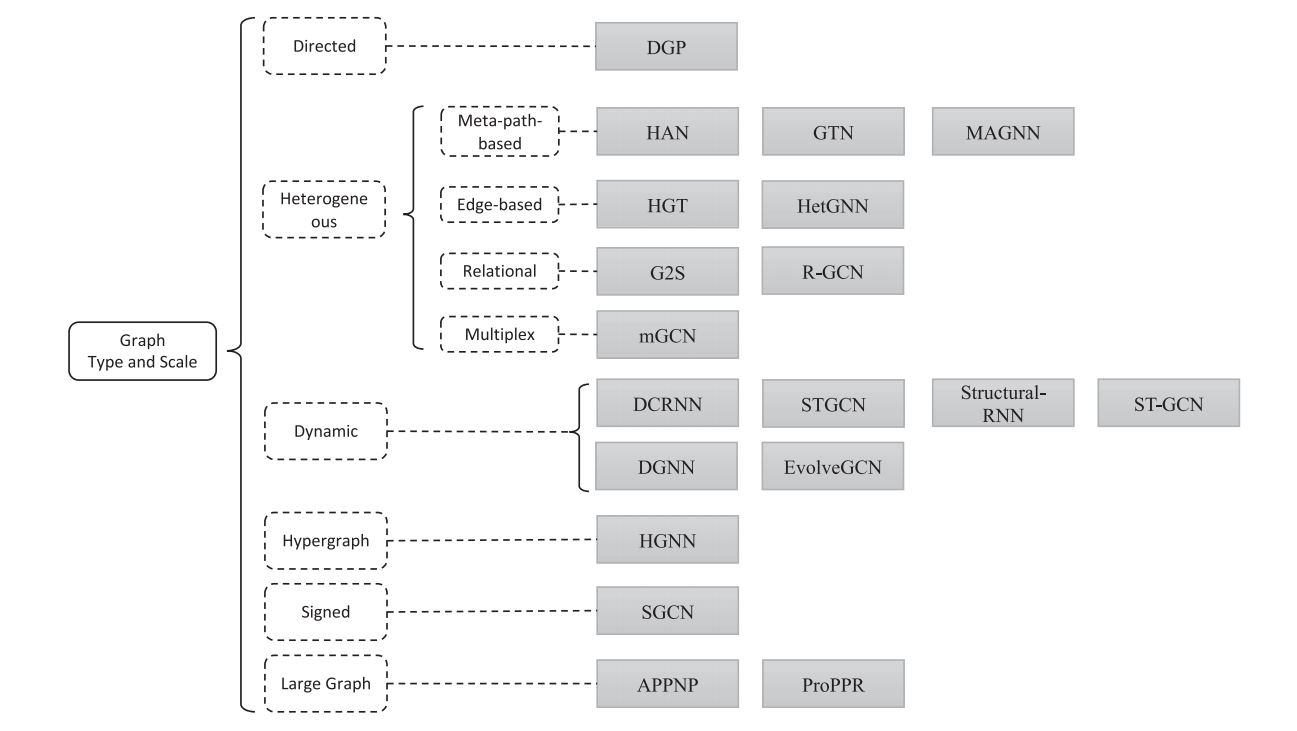
\includegraphics[scale=0.5]{6.png}
			\caption{不同的图结构}
			\label{fig:label}
		\end{figure}
		
		有向图(Directed Graphs): 无向边可以看成是两个有向边的结合,但是,有向边比无向边能够 提供更多的信息,比如在知识图谱里面,边开始于头实体(head entity),结束于尾实体(tail entity).
		\citep{conf/Michael2019}使用两种权重矩阵和来结合更加精确的结构化信息,DGP的传播方式如下:
		$$
		\mathbf{H}^{t}=\sigma\left(\mathbf{D}_{p}^{-1} \mathbf{A}_{p} \sigma\left(\mathbf{D}_{c}^{-1} \mathbf{A}_{c} \mathbf{H}^{t-1} \mathbf{W}_{c}\right) \mathbf{W}_{p}\right)
		$$
		其中, $\mathbf{D}_{p}^{-1} \mathbf{A}_{p}$ 和 $\mathbf{D}_{c}^{-1} \mathbf{A}_{c}$ 分别是双亲(parents)和后代(children)的归一化邻接矩阵。
		- 异质图(Heterogeneous Graphs):异质图含有多种不同的节点种类,处理这种图最简单的方 法是将每种节点的类型转化为One-hot特征向量,然后将One-hot向量和原始的节点特征进行
		连接,作为该节点的特征向量。其中,\citep{conf/YizhouZhang2018}提出将元路径(metapath)概念用在 异质图的信息传播上,通过元路径的方式,我们可以根据节点类型和距离来对局部范围内节点进 行分组,对于每一组,Graphlnception将它作为异质图的一个子图,然后在子图内进行传播, 并将不同异质图得到的结果进行连接得到综合的节点表示。
		- 带有边信息的图(Graphs with Edge Information):在这种图变体中,每一个边都带有额外的 信息,比如权重和边的类型,我们可以使用两种方法来处理这种图:
		一种方式是将原始的图转化为一个二分图(bipartite graph),处理方式为将原始的边转化为一个 节点以及两条新的边,\citep{conf/DanielBeck2018} 的编码器使用如下的传播函数:
		$$
		\mathbf{h}_{v}^{t}=\rho\left(\frac{1}{\left|\mathcal{N}_{v}\right|} \sum_{u \in \mathcal{N}_{v}} \mathbf{W}_{r}\left(\mathbf{r}_{v}^{t} \odot \mathbf{h}_{u}^{t-1}\right)+\mathbf{b}_{r}\right)
		$$
		其中, $\mathbf{W}_{r}$ 和 $\mathbf{b}_{r}$ 是不同边类型的传播参数。
		另一种方式是在不同种类的边上,使用不同的权重矩阵来进行传播的方式,也就是说,每一种边 类型都关联一个权重矩阵,显然,对于边类型有很多的情况下,这种方式的参数量会非常大,\citep{conf/Schlichtkrull2018}采用两种方法来减小参数。
		- 动态图(Dynamic Graphs):动态图类型有静态的图结构,并且能够处理动态的输入信号。 DCRNN和STGCN首先使用GNN获取空域信息,然后将该信息输入到一个序列模型,比如 sequence-to-sequence模型或者CNN模型。与此相反的是,Structural-RNN和ST-GCN同时 获取时间信息和空间信息。
		
		
		\subsection{不同的GNN传播机制}
		图神经网络中的传播(propagation)指的是汇集从邻居节点和连接的边的信息,来对节点进行更新的过程,这个过程在模型中获取节点(或边)的隐藏状态是非常重要的。对于信息传播步骤(propagation step),有几种主要的GNN变体,而在输出步骤(output step)中,研究者通常使用简单的前向传播的神经网络。
		
		图的节点更新的主要信息传播(information aggregator)类型以及主要的模型如下图:
		\begin{figure}[ht]
			\centering
			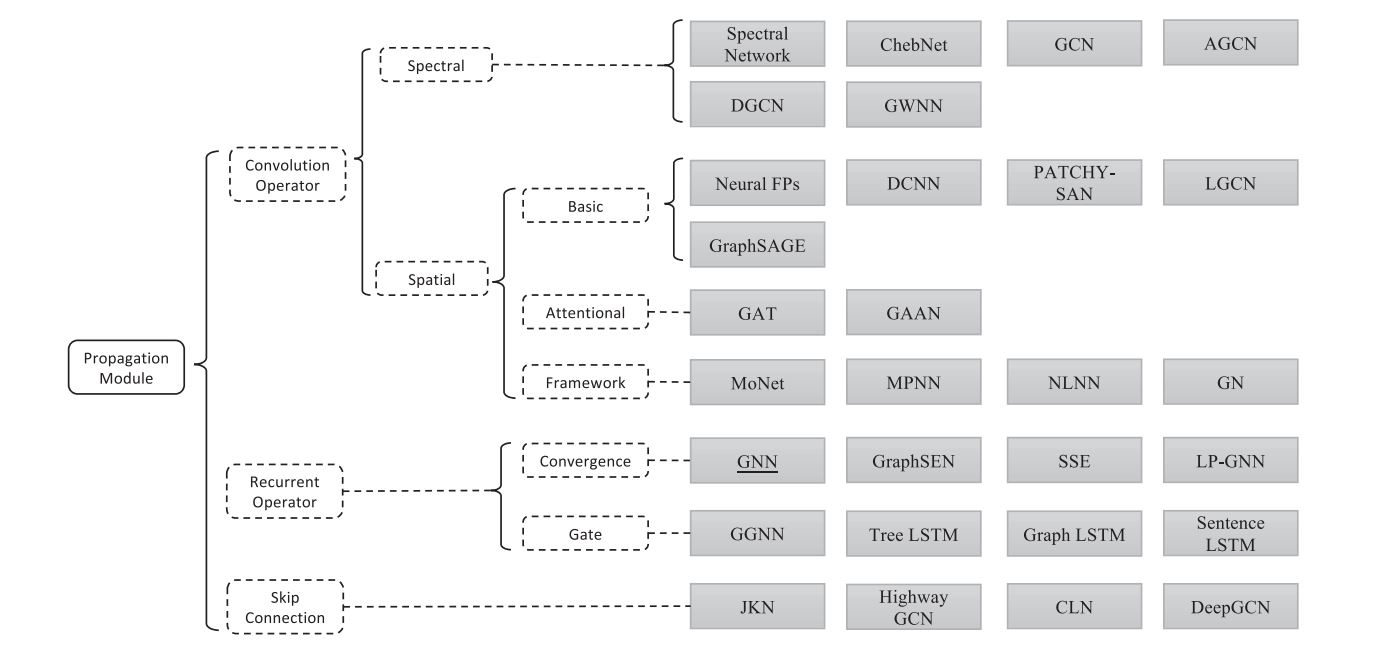
\includegraphics[scale=0.5]{7.png}
			\caption{不同的GNN传播方式}
			\label{fig:label}
		\end{figure}
		
		1. 卷积(Convolution): 这个方向上分为频域方法和非频域(空域)方法。
		$\Rightarrow>>>$ 频掝方法使用图的频域表示,主要有以下几种模型:
		Spectral Network: \citep{conf/Thomas2017}提出了Spectral network,卷积操作定义为傅里叶频域计算图拉普拉斯(graph Laplacian)的特征值分解。这个操作可以定义为使用卷积核 $\mathrm{g}_{0}=\operatorname{diag}(\theta)$ 对输入 $\mathbf{x} \in \mathbb{R}^{N}$ (每一个节点有一个标量值)的卷积捛作,其中 $\theta \in \mathbb{R}^{N}$
		
		$$
		\mathbf{g}_{\theta} \star \mathbf{x}=\mathbf{U}_{\theta}(\boldsymbol{\Lambda}) \mathbf{U}^{T} \mathbf{x}
		$$
		其中, $\mathrm{U}$ 是标准化图拉普拉斯矩阵 $\mathbf{L}=\mathbf{I}_{N}-\mathbf{D}^{-\frac{1}{2}} \mathbf{A D}^{-\frac{1}{2}}=\mathbf{U} \mathbf{\Lambda} \mathbf{U}^{T}$ 的特征向量矩 阵, $\mathbf{D}$ 是度矩阵(degree matrix), $\mathbf{A}$ 是图的邻唼矩阵(adjacency matrix), $\mathbf{\Lambda}$ 为以特征 值为对角线上的值的对角矩阵。这个操作会有导致较高的计算量。
		
		ChebNet: \citep{journal/JieZhou2020}根据切比雪夫多项式定理,认为 $\mathrm{g}_{0}(\boldsymbol{\Lambda})$ 可以通过取多项式的前 $K$ 项来进 行估计,因此,操作为
		$$
		\mathbf{g}_{\theta} \star \mathbf{x} \approx \mathbf{U} \sum_{k=0}^{K} \theta_{k} \mathbf{T}_{k}(\tilde{\mathbf{L}}) \mathbf{U}^{\mathbf{T}} \mathbf{x}
		$$
		其中, $\tilde{\mathbf{L}}=\frac{2}{\lambda_{\max }} \mathbf{L}-\mathbf{I}_{N} , \lambda_{\max }$ 表示矩阵 $\mathbf{L}$ 最大的特征值, $\theta \in \mathbb{R}^{K}$ 为切比雪夫 系数向量,切比雪夫多项式定义为 $\mathbf{T}_{k}(\mathbf{x})=2 \mathbf{x} \mathbf{T}_{k-1}(\mathbf{x})-\mathbf{T}_{k-2}(\mathbf{x})$ ,且有 $\mathbf{T}_{0}(\mathbf{x})=1$ 以及 $\mathbf{T}_{1}(\mathbf{x})=\mathbf{x}$ 。可以看出,这个操作是 K-localized,因为在拉普拉斯中 它是一个K阶终项式。由此避免了计算拉晋拉斯的特征值。
		GCN : \citep{conf/Thomas2017}限制了逐层的卷积操作,并设置  K=1 \text { 来咸䌽过拟合的问题,近似了 }
		$\lambda_{\max } \approx 2$, 最后简化的方程如下
		$$
		\mathbf{g}_{\theta^{\prime}} \star \mathbf{x} \approx \theta_{0}^{\prime} \mathbf{x}+\theta_{1}^{\prime}\left(\mathbf{L}-\mathbf{I}_{N}\right) \mathbf{x}=\theta_{0}^{\prime} \mathbf{x}-\theta_{1}^{\prime} \mathbf{D}^{-\frac{1}{2}} \mathbf{A} \mathbf{D}^{-\frac{1}{2}} \mathbf{x}
		$$
		使用两个无限制的参数 $\theta_{0}^{\prime}$ 和 $\theta_{1}^{\prime}$ 。在通过设置 $\theta=\theta_{0}^{\prime}=-\theta_{1}^{\prime}$ 来限制参数的数量之后,我 们可以得到一下的表达式
		$$
		\mathbf{g}_{\theta} \star \mathbf{x} \approx \theta\left(\mathbf{I}_{N}+\mathbf{D}^{-\frac{1}{2}} \mathbf{A} \mathbf{D}^{-\frac{1}{2}}\right) \mathbf{x}
		$$
		值得一提的是,受加使用这个操作会导致数值不稳定性以及梯度爆炸或消失(因为不断地乘以同 一个矩阵),因此,该论文里面使用了重规整化操作(renormalization):
		$$
		\mathbf{I}_{N}+\mathbf{D}^{-\frac{1}{2}} \mathbf{A D}^{-\frac{1}{2}} \rightarrow \tilde{\mathbf{D}}^{-\frac{1}{2}} \tilde{\mathbf{A}} \tilde{\mathbf{D}}^{-\frac{1}{2}}
		$$
		其中 $\tilde{\mathbf{A}}=\mathbf{A}+\mathbf{I}_{N} , \tilde{\mathbf{D}}_{i i}=\sum_{j} \tilde{\mathbf{A}}_{i j}$ ,最后,论文将模型扩展为含有 $C$ 个输入通道的 信昊 $\mathbf{X} \in \mathbb{R}^{N \times C}$ 以及 $F$ 个滤波嘲来用于提取特征
		$$
		\mathbf{Z}=\tilde{\mathbf{D}}^{-\frac{1}{2}} \tilde{\mathbf{A}} \tilde{\mathbf{D}}^{-\frac{1}{2}} \mathbf{X} \boldsymbol{\Theta}
		$$
		
		其中, $\Theta \in \mathbb{R}^{C \times F}$ 是滤波㽞参数矩阵, $\mathbf{Z} \in \mathbb{R}^{N \times F}$ 是卷积信昊矩阵。
		在所有这些频域方法中,学习得到的滤波器都是其于拉普拉斯牛佂分解,也訧是取决于图的结 构,这也就意味着,在一个特定结构上训练得到的模型,井不能直接应用到另外一个结构不同的 图上。
		$\gg>>$ 非频域的方法直接在图上定义卷积操作,也就是在空域上相阾的邻居节点上进行操 作。这种非频域方法的主要难点在于如何定义拥有不同邻居数量的卷积操作以及保持CNN的局 部不变性。主要的模型有如下一些:
		Neural FPs: \citep{conf/David2015}对不同度的节点使用不同的权重矩阵
		$$
		\begin{aligned}
			&\mathbf{x}=\mathbf{h}_{v}^{t-1}+\sum_{i=1}^{\left|\mathcal{N}_{v}\right|} \mathbf{h}_{i}^{t-1} \\
			&\mathbf{h}_{v}^{t}=\sigma\left(\mathbf{x}_{t}^{\left|\mathcal{N}_{v}\right|}\right)
		\end{aligned}
		$$ 到节点度比较大的graph上。
		论文的应用场景是分子指纹(Molecular Fingerprints)领域,通过图神经网络的方式来学习分 子表示,从而提供下游任务比如相似度评估任务或分类任务需要的向量表示。
		
		DCNN: \citep{conf/James2016}提出了扩散卷积神经网絡,转化矩阵用来定义节点的邻㕆,对于节点分关任务, 有
		$$
		\mathbf{H}=f\left(\mathbf{W}^{c} \odot \mathbf{P}^{*} \mathbf{X}\right)
		$$
		其中, $\mathbf{X}$ 是一个 $N \times F$ 的输入特征张量 ( $N$ 是节点的数量, $F$ 是特佂的维度), $\mathbf{P}^{*}$ 是一个 $N \times K \times N$ 的张量,包念矩阵 $\mathbf{P}$ 的power series $\left\{\mathbf{P}, \mathbf{P}^{2}, \ldots, \mathbf{P}^{K}\right\} , \mathbf{P}$ 是来自于图邻接矩阵 $\mathbf{A}$ 的度标准(degree-normalized)的转化矩阵。
		
		DGCN:\citep{journal/JieZhou2020}提出了对偶图卷积网紟,同时考虑到图上的局部一攻性和全局一致性,它使用两 组卷积网络来获取局部/全局的一致性,并采用一个无监督的loss来姐合它们,第一个卷积网絡 和方程相同,第二个卷积网络将邻接矩阵凿换为PPMI(positive pointwise mutual information)矩阵
		$$
		\mathbf{H}^{\prime}=\rho\left(\mathbf{D}_{P}^{-\frac{1}{2}} \mathbf{X}_{P} \mathbf{D}_{P}^{-\frac{1}{2}} \mathbf{H} \Theta\right)
		$$
		其中, $\mathbf{X}_{P}$ 为PPMI矩阵, $\mathbf{D}_{P}$ 为 $\mathbf{X}_{P}$ 的对角度矩阵。
		GraphSAGE: \citep{journal/JieZhou2020}提出了一个一般的归纳框架,这个框架通过从一个节点的局部阾居中采样和 聚合特征,来产生节点的embedding
		$$
		\mathbf{h}_{\mathcal{N}_{v}}^{t}=\text { AGGREGATE }{ }_{t}\left(\left\{\mathbf{h}_{u}^{t-1}, \forall u \in \mathcal{N}_{v}\right\}\right)
		$$
		
		$$
		\mathbf{h}_{v}^{t}=\sigma\left(\mathbf{W}^{t} \cdot\left[\mathbf{h}_{v}^{t-1} \| \mathbf{h}_{N_{v}}^{t}\right]\right)
		$$
		但是,上述的方程并不会采用所有的邻居节点进行计算,而是使用均匀采样来得到固定大小的邻 居节点集合,该论文推荏使用三种聚合函数:
		(1)平均值聚合(Mean aggregator):使用如下方式计算
		$$
		\mathbf{h}_{v}^{t}=\sigma\left(\mathbf{W} \cdot \operatorname{MEAN}\left(\left\{\mathbf{h}_{v}^{t-1}\right\} \cup\left\{\mathbf{h}_{u}^{t-1}, \forall u \in \mathcal{N}_{v}\right\}\right)\right.
		$$
		平均值聚合和其他的聚合方式不同,因为它不用进行连接操作。
		(2)LSTM聚合(LSTM aggregator):其于LSTM的聚合唶有更好的表达能力,然而,LSTM以序 列的方式顺序地处理输入,因此,它井没有排列不变性,论文采用重排列节点邻居的方式,在无 序集合中使用LSTM操作。
		(3)池化聚合(Pooling aggregator):每一个令居的隐藏状态输入到一个全连接层,然后使用最 大池化操作应用到邻居节点集合。
		$$
		\mathbf{h}_{N_{v}}^{t}=\max \left(\left\{\sigma\left(\mathbf{W}_{\text {pool }} \mathbf{h}_{u}^{t-1}+\mathbf{b}\right), \forall u \in \mathcal{N}_{v}\right\}\right)
		$$
		值得一提的是,任何对称的函数都可以用来萆换这里的最大池化操作。
		2. 门机制(Gate): 目前在信息传播步裂中使用的门机制类似于GRU和LSTM模型,这种机制可以减 小原始GNN模型的约束,并提升在图结构中的长期的信息传播。
		
		GGNN: \citep{conf/YujiaLi2016}提出了门控图神经网絡(GGNN),在信息传播步骤中使用GRU,将递归循坏展开 固定数量的步数,并使用按照时间序的反向传播来计算梯度。
		具体来说,传播的基本递归循环是模型如下
		$\mathbf{a}_{v}^{t}=\mathbf{A}_{v}^{T}\left[\mathbf{h}_{1}^{t-1} \ldots \mathbf{h}_{N}^{t-1}\right]^{T}+\mathbf{b}$
		$\mathbf{z}_{v}^{t}=\sigma\left(\mathbf{W}^{z} \mathbf{a}_{v}^{t}+\mathbf{U}^{z} \mathbf{h}_{v}^{t-1}\right)$
		$\mathbf{x}_{v}^{t}=\sigma\left(\mathbf{W}^{r} \mathbf{a}_{v}^{t}+\mathbf{U}^{r} \mathbf{h}_{v}^{t-1}\right)$
		$\widetilde{\mathbf{h}}_{v}^{t}=\tanh \left(\mathbf{W} \mathbf{a}_{v}^{t}+\mathbf{U}\left(\mathbf{r}_{v}^{t} \odot \mathbf{h}_{v}^{t-1}\right)\right)$
		$\mathbf{h}_{v}^{t}=\left(1-\mathbf{z}_{v}^{t}\right) \odot \mathbf{h}_{v}^{t-1}+\mathbf{z}_{v}^{t} \odot \widetilde{\mathbf{h}_{v}^{t}}$
		按照第一个公式,节点 $v$ 首先从它的邻居节点汇集信息,其中, $\mathbf{A}_{v}$ 为图邻唼矩阵 $\mathbf{A}$ 的子矩 阵,表示节点 $v$ 和它的邻居节点的连接关系。然后,关似于GRU的节点更新函数将该节点前一 个时刻的信息和与该节点相邻的其它节点的信息结合起来,以此来更新每一个节点的隐藏状 态。 $\mathbf{a}$ 汇集了节点 $v$ 周围节点的信息, $\mathbf{z}$ 和 $\mathbf{r}$ 分别是更新门(update gate)和重置门] (reset gate)。LSTM同样使用关似的方法来进行信息传㨨过程。
		
		Tree-LSTM: \citep{journal/JieZhou2020}提出了两个LSTM的扩展結构,Child-Sum Tree-LSTM和N-ary TreeLSTM,类似于标准的LSTM单元,每一个Tree-LSTM单元(为)包念输入门(input gate)和输出门 (output gate),记忆单元(memory cell)和隐藏状态(hidden state),但与LSTM(LSTM单元只 包含一个遗忘门'(forget gate))不同的是,Tree-LSTM单元对每一个孩子节点都有一个遗忘门] ,这样就可以从孩子节点中选择性地汇集茾组合信息。Child-Sum Tree-LSTM的转换方程如下
		
		$$
		\begin{aligned}
			\widetilde{\mathbf{h}_{v}^{t-1}} &=\sum_{k \in \mathcal{N}_{v}} \mathbf{h}_{k}^{t-1} \\
			\mathbf{i}_{v}^{t} &=\sigma\left(\mathbf{W}^{i} \mathbf{x}_{v}^{t}+\mathbf{U}^{i} \widetilde{\mathbf{h}_{v}^{t-1}}+\mathbf{b}^{i}\right) \\
			\mathbf{f}_{v k}^{t} &=\sigma\left(\mathbf{W}^{f} \mathbf{x}_{v}^{t}+\mathbf{U}^{f} \mathbf{h}_{k}^{t-1}+\mathbf{b}^{f}\right) \\
			\mathbf{o}_{v}^{t} &=\sigma\left(\mathbf{W}^{o} \mathbf{x}_{v}^{t}+\mathbf{U}^{o} \mathbf{h}_{v}^{t-1}+\mathbf{b}^{o}\right) \\
			\mathbf{u}_{v}^{t} &=\tanh \left(\mathbf{W}^{u} \mathbf{x}_{v}^{t}+\mathbf{U}^{u} \mathbf{h}_{v}^{t-1}+\mathbf{b}^{v}\right) \\
			\mathbf{c}_{v}^{t} &=\mathbf{i}_{v}^{t} \odot \mathbf{u}_{v}^{t}+\sum_{k \in \mathcal{N}_{v}} \mathbf{f}_{v k}^{t} \odot \mathbf{c}_{k}^{t-1} \\
			\mathbf{h}_{v}^{t} &=\mathbf{o}_{v}^{t} \odot \tanh \left(\mathbf{c}_{v}^{t}\right)
		\end{aligned}
		$$
		$\mathbf{x}_{v}^{t}$ 是标准LSTM中在时刻 $t$ 的输入。
		如果一个树每一个节点最多有 $K$ 个分支,并且节点所有的孩子节点都是有序的,比如,这些 孩子节点可以被从 1 编旦到 $X$ ,那么可以使用 $N$-ary Tree-LSTM,对于节点 $v , \mathbf{h}_{v k}^{t}$ 和 $\mathbf{c}_{v k}^{t}$ 分别表示在 $t$ 时刻,它的第 $k$ 个孩子节点的隐葳状态和记忆单元,转化方程为
		$$
		\begin{aligned}
			\mathbf{i}_{v}^{t} &=\sigma\left(\mathbf{W}^{i} \mathbf{x}_{v}^{t}+\sum_{l=1}^{K} \mathbf{U}_{i}^{i} \mathbf{h}_{v l}^{t-1}+\mathbf{b}^{i}\right) \\
			\mathbf{f}_{v k}^{t} &=\sigma\left(\mathbf{W}^{f} \mathbf{x}_{v}^{t}+\sum_{l=1}^{K} \mathbf{U}_{k l}^{f} \mathbf{h}_{v l}^{t-1}+\mathbf{b}^{f}\right) \\
			\mathbf{o}_{v}^{t} &=\sigma\left(\mathbf{W}^{o} \mathbf{x}_{v}^{t}+\sum_{l=1}^{K} \mathbf{U}_{l}^{o} \mathbf{h}_{v l}^{t-1}+\mathbf{b}^{o}\right) \\
			\mathbf{u}_{v}^{t} &=\tanh \left(\mathbf{W}^{u} \mathbf{x}_{v}^{t}+\sum_{l=1}^{K} \mathbf{U}_{v l}^{t} \odot \mathbf{c}_{v i}^{t-1}+\mathbf{b}^{t h}\right) \\
			\mathbf{c}_{v}^{t} &=\mathbf{i}_{v}^{t} \odot \mathbf{u}_{v}^{t}+\sum_{l=1}^{K} \mathbf{f}_{v l}^{t} \odot \mathbf{c}_{v l}^{t-1} \\
			\mathbf{h}_{v}^{t} &=\mathbf{o}_{v}^{t} \odot \tanh \left(\mathbf{c}_{v}^{t}\right)
		\end{aligned}
		$$
		对每个孩子节点 $k$ 都恜予一个单独的参数矩阵,使得该模型相比于Child-Sum Tree-LSTM能 够学习得到更加细微的节点表示。这两种关型的Tree-LSTM都能驹很容易地应用到图。
		\citep{journal/JieZhou2020}提出了一个Graph LSTM的变体,用于关系抽取(relation extraction)的任务上。图和树的 主要区别在于,图结构的边有它们自己的label,由此,\citep{journal/JieZhou2020}采用不同的权重矩阵来表示不同的 label
		$$
		\begin{aligned}
			\mathbf{i}_{v}^{t} &=\sigma\left(\mathbf{W}^{i} \mathbf{x}_{v}^{t}+\sum_{k \in \mathcal{N}_{v}} \mathbf{U}_{m(v, k)}^{i} \mathbf{h}_{k}^{t-1}+\mathbf{b}^{i}\right) \\
			\mathbf{f}_{v k}^{t} &=\sigma\left(\mathbf{W}^{f} \mathbf{x}_{v}^{t}+\mathbf{U}_{m(v, k)}^{f} \mathbf{h}_{k}^{t-1}+\mathbf{b}^{f}\right) \\
			\mathbf{o}_{v}^{t} &=\sigma\left(\mathbf{W}^{o} \mathbf{x}_{v}^{t}+\sum_{k \in \mathcal{N}_{v}} \mathbf{U}_{m(v, k)}^{o} \mathbf{h}_{k}^{t-1}+\mathbf{b}^{o}\right) \\
			\mathbf{u}_{v}^{t} &=\tanh \left(\mathbf{W}^{u} \mathbf{x}_{v}^{t}+\sum_{k \in \mathcal{N}_{v}} \mathbf{U}_{m(v, k)}^{t-1} \mathbf{h}_{k}^{t-1}+\mathbf{b}^{u}\right) \\
			\mathbf{c}_{v}^{t} &=\mathbf{i}_{v}^{t} \odot \mathbf{u}_{v}^{t}+\sum_{k \in \mathcal{N}_{v}} \mathbf{f}_{v k}^{t} \odot \mathbf{c}_{k}^{t-1} \\
			\mathbf{h}_{v}^{t} &=\mathbf{o}_{v}^{t} \odot \tanh \left(\mathbf{c}_{v}^{t}\right)
		\end{aligned}
		$$
		其中, $m(v, k)$ 表示在节点 $v$ 和 $k$ 之间边的label。
		
		\section{可自由添加后续章节}
		
		%% 参考文献列表  参考文献位于 ref.bib 中, 文件中给出了书籍 期刊 会议的格式, 请参照对应格式添加参考文献
		\bibliographystyle{abbrvnat}
		\bibliography{ref}
	\end{document}
	
	使用\textbackslash{}citep 命令引用参考文献,  例如\citep{book/mohri2018foundations} \citep{journal/Vapnik1971} \citep{conf/Sugiyama2006local}